\documentclass[12pt]{article}
\usepackage[margin=1.5cm]{geometry}
\usepackage{parskip}
\usepackage{amsmath}
\usepackage{amssymb}
\usepackage{amsfonts}
\usepackage{enumitem}
\usepackage{graphicx}
\usepackage{stmaryrd}
\graphicspath{ {./images/} }


\begin{document}
\begin{enumerate}[label=(\alph*)]

  \item

    We perform scheduling over basic blocks. We detail the actions that are sensibly taken at boundaries of sequential code at the end, once the scheduling algorithm has been described.

    We propose the following scheduling algorithm:

    \begin{itemize}
        \item
          Build a DAG from the instructions in our basic block, such that:

          A node is created for each instruction.

          An edge from $n$ to $n'$ exists if $n$ occurs before $n'$ in the original program order, and there is a dependency between $n$ and $n'$ ($n$ reads from a register $n'$ writes to, $n$ writes to a register that $n'$ reads from, or $n$ and $n'$ both write to the same register).

          \item
            Construct a set of instructions that can be scheduled, initialised as those nodes with no predecessors.

            \item
              While that set is not empty, choose an instruction to schedule that satisfies the following heuristics:

              \begin{itemize}
                  \item
                    Prefer an instruction that does not conflict with the previous instruction.

                    \item
                      Prefer an instruction that is more likely to cause conflicts (e.g. loads over adds)

                      \item
                        Prefer an instruction that is furthest away from a final node, along the longest path (where `final' node is any node that can be scheduled last, i.e. has no successors).
              \end{itemize}

              The first heuristic cannot be always satisfied, but the other two can because they are comparative.

              The first heuristic obviously does no harm to satisfy, and only improves performance.

              The second heuristic allows us to try and avoid having to not satisfy the first heuristic.

              The third heuristic attempts to interleave independent instruction streams, such that we can avoid stalls through interleaving.

              \item
                After scheduling an instruction, remove it from the set of instructions to schedule and the DAG, and if any of its successors no longer have any predecessors, add them to the set of instructions to schedule.
    \end{itemize}

    Since our hardware is interlocked, we do not have any correctness issues at boundaries between basic blocks, although for performance, we should consider the final instructions in each of the scheduled predecessor flowgraphs, and if any of them are load instructions, then we should take this into account when scheduling our first instruction and try to avoid a conflict where possible.

    \item
      We number the instructions as follows:

\begin{verbatim}
1: ldr r3,[r1,#0]
2: str r3,[r2,#0]
3: ldr r4,[r1,#4]
4: str r4,[r2,#4]
5: add r5,r4,#4
\end{verbatim}

We get the following DAG:

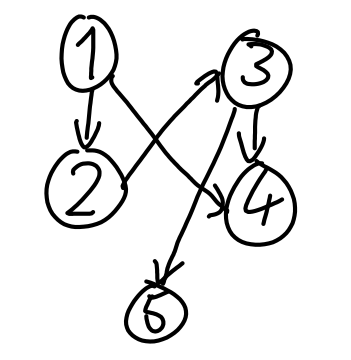
\includegraphics[scale=0.5]{dag}

Since load and store instructions access memory, and we do not know the values of $r1$ and $r2$, we consider that all loads must occur before future stores, and all stores must occur before future loads and stores (unless we can infer that the two accesses go to different locations, like we can between instructions 2 and 4, assuming a 32-bit system).

So, we must emit instruction 1 at the start, since it is the only instruction with no predecessors.

Then, we must emit instruction 2, since it is the only instruction with no predecessors.

Then, we must emit instruction 3, since it is the only instruction with no predecessors.

Finally, we have a choice between instruction 4 and 5. We choose instruction 4, since instruction 5 conflicts with instruction 3 (load-use delay), and then we must schedule instruction 5, so we end with the schedule [1,2,3,4,5]. This in total takes 7 cycles to execute (2 load-use delays between loads and stores).

If we assume that $r1$ and $r2$ do not alias, then we get the following DAG:

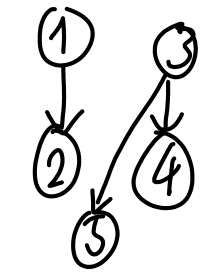
\includegraphics[scale=0.5]{dag2}

In this case, we do the following scheduling:

We can schedule either instruction 1 or 3, we schedule 1 arbitrarily since both instructions fit all 3 heuristics.

Then we can schedule either instruction 2 or 3. We schedule instruction 3 since it does not conflict with the previous store instruction.

Then, we can schedule either instruction 2, 4, or 5. We  schedule instruction 2 since it is the only one that does not conflict with the previous instruction.

Then, we can schedule either instruction 4 or 5. We choose instruction 5, since instruction 4 will conflict with the previous store.

Finally, we schedule instruction 4.

This takes 5 cycles to execute (no load-use or store-store delays).

\item
  We number the instructions:

\begin{verbatim}
1: add r3,r1,r2
2: or  r4,r1,r2
3: sub r5,r3,r4
4: xor r4,r1,r3
\end{verbatim}

Clearly, we must schedule instructions 1 and 2 before instruction 3, since instruction 3 uses those results. Furthermore, we must schedule instruction 4 after instructions 1 and 2, since it has a RAW dependency with instruction 1, and a WAW dependency with instruction 2. We must also schedule instruction 4 after instruction 3 since it has a WAR dependency with it.

Therefore, instruction 4 must be the last instruction, instructions 1 and 2 must be the first two instructions, and thus we have no choice for instruction 3.

Therefore, we only get the two schedulings [1,2,3,4] and [2,1,3,4].

  
        
    \end{enumerate}
\end{document}
